\documentclass[10pt,a4paper,twocolumn]{article}
\usepackage[utf8]{inputenc}
\usepackage[T1]{fontenc}
% babel em português quando disponível (Overleaf tem)
\IfFileExists{portuguese.ldf}{\usepackage[brazil]{babel}}{%
  \AtBeginDocument{\renewcommand{\tablename}{Tabela}\renewcommand{\figurename}{Figura}}}
\usepackage{mathptmx}
\usepackage[margin=1.7cm,top=1.5cm,bottom=1.6cm]{geometry}
\usepackage{booktabs,graphicx,xcolor,amsmath}
\usepackage[hidelinks]{hyperref}
\usepackage{titlesec,enumitem}
\setlength{\columnsep}{0.6cm}
\titlespacing*{\section}{0pt}{6pt}{3pt}
\titleformat*{\section}{\large\bfseries}
\setlist{nosep,leftmargin=*}
\setlength{\parskip}{2pt}

% Campos a preencher após rodar o notebook (aparecem em laranja no PDF).
% Para a versão final, troque cada \preencher{...} pelo valor.
\newcommand{\preencher}[1]{\textcolor{orange!85!black}{\textbf{[#1]}}}

\title{\vspace{-1.2cm}\Large U-Net treinada do zero para segmentação semântica urbana:\\
um estudo de ablação no CamVid\\[2pt]
\normalsize Relatório de progresso --- \preencher{Disciplina}}
\author{Elder \preencher{sobrenome} \quad ---\quad \preencher{programa / instituição}}
\date{24 de outubro de 2026}

\begin{document}
\maketitle
\vspace{-0.8cm}

\section{Problema e perguntas de pesquisa}
Segmentação semântica atribui uma classe a cada pixel da imagem. Estudamos a U-Net
\cite{ronneberger} treinada \emph{sem pré-treino}, num dataset pequeno e desbalanceado,
para isolar o que cada componente do projeto contribui quando não há representações
prontas a herdar. Cada pergunta é respondida variando \emph{um único fator}
em relação a um baseline:
\begin{enumerate}
  \item[\textbf{Q1}] \textbf{Arquitetura:} quanto do desempenho vem das \emph{skip
  connections}? Hipótese: sem elas o modelo perde detalhes espaciais, e a queda se
  concentra nas classes finas (poste, placa, ciclista).
  \item[\textbf{Q2}] \textbf{Desbalanceamento:} ponderar a cross-entropy por classe ou
  somar a perda Dice \cite{milletari} melhora o mIoU? Hipótese: ganho nas classes raras,
  com possível perda leve nas dominantes.
  \item[\textbf{Q3}] \textbf{Regularização:} qual o efeito de data augmentation com
  apenas 367 imagens de treino? Hipótese: sem augmentation há mais overfitting
  (maior distância entre loss de treino e mIoU de validação).
  \item[\textbf{Q4}] \textbf{Capacidade} (opcional): como o mIoU varia com a largura
  da rede (1,9M, 7,8M e 31M parâmetros)?
\end{enumerate}

\section{Dataset e justificativa da escolha}
O \textbf{CamVid} \cite{camvid} contém frames de vídeo urbano anotados com 11 classes
(mais \emph{Void}, ignorada). Usamos a divisão do SegNet \cite{segnet}: 367 imagens de
treino, 101 de validação e 233 de teste, em 360$\times$480.
Motivos da escolha:
\begin{itemize}
  \item \textbf{Viável do zero no orçamento:} é pequeno o bastante para cada treino
  levar minutos em uma GPU do Colab, o que permite várias variantes e seeds.
  \item \textbf{Multiclasse e desbalanceado} (Tab.~\ref{tab:classes}): \emph{Road}
  ocupa 31,7\% dos pixels e \emph{Bicyclist} 0,29\% (razão $\approx$110$\times$).
  Isso torna Q1 e Q2 informativas, ao contrário de datasets binários e fáceis
  (ex.: Carvana, onde as variantes saturam perto de Dice 0,99).
  \item \textbf{Divisão padronizada e amplamente usada}, o que permite comparar
  ordens de grandeza com a literatura.
  \item Domínio fora da saúde e sem cadastro para download (ao contrário do Cityscapes).
\end{itemize}

\begin{table}[h]
\centering\small
\caption{Fração dos pixels de treino por classe (calculada nas 367 anotações).}
\label{tab:classes}
\setlength{\tabcolsep}{4pt}
\begin{tabular}{lr@{\hskip 14pt}lr}
\toprule
Classe & \% & Classe & \% \\
\midrule
Road & 31,66 & Car & 5,87 \\
Building & 23,26 & Pavement & 4,49 \\
Sky & 16,85 & SignSymbol & 1,17 \\
Tree & 9,72 & Fence & 1,13 \\
Void (ign.) & 3,95 & Pole & 0,98 \\
 & & Pedestrian & 0,64 \\
 & & Bicyclist & 0,29 \\
\bottomrule
\end{tabular}
\end{table}

\section{Metodologia}
\textbf{Modelo.} U-Net com 4 níveis de \emph{downsampling}, blocos
conv3$\times$3--BN--ReLU duplos, \emph{upsampling} por convolução transposta e largura
base de 32 filtros (32$\rightarrow$512; $\approx$\preencher{7,8}M parâmetros). Na
variante sem skip, o decodificador recebe apenas o mapa reamostrado.

\textbf{Treino.} AdamW (lr $10^{-3}$, weight decay $10^{-4}$), \emph{cosine annealing},
120 épocas, batch 8, precisão mista. Recortes aleatórios de 256$\times$256 em todas as
variantes; augmentation = flip horizontal + brilho/contraste. Pesos da CE ponderada por
\emph{median frequency balancing} \cite{eigen}.

\textbf{Protocolo.} Seleção do checkpoint pelo mIoU de validação (avaliado a cada 2
épocas); conjunto de teste avaliado \emph{uma única vez}, na imagem inteira.
\textbf{Métricas:} mIoU (principal), IoU por classe e acurácia de pixel, com
média $\pm$ desvio-padrão sobre 3 seeds.

\section{Plano de experimentos}
\begin{table}[h]
\centering\small
\caption{Variantes (cada uma muda um fator do baseline), 3 seeds cada.}
\label{tab:plano}
\begin{tabular}{llc}
\toprule
Variante & Alteração & Pergunta \\
\midrule
baseline & U-Net-32, CE, com aug. & --- \\
no\_skip & sem skip connections & Q1 \\
wce & CE ponderada & Q2 \\
ce\_dice & CE + Dice & Q2 \\
no\_aug & sem augmentation & Q3 \\
base16 / base64 & largura 16 / 64 & Q4 \\
\bottomrule
\end{tabular}
\end{table}

\textbf{Orçamento.} Medido no smoke test: \preencher{X} s/época em GPU
\preencher{L4}, ou $\approx$\preencher{Y} min por treino. As 5 variantes prioritárias
$\times$ 3 seeds somam $\approx$\preencher{15$\times$Y} min; Q4 roda se houver saldo de
unidades de computação.

\textbf{Análises previstas:} tabela de mIoU (média $\pm$ dp); IoU por classe, com foco nas
classes raras; curvas de treino e validação (overfitting, Q3); exemplos qualitativos dos
melhores e piores casos.

\section{Código}
Repositório: \url{https://github.com/SEU_USUARIO/unet-camvid} \preencher{atualizar link}.
Uma função \texttt{run(Config)} treina qualquer variante, registra curvas em CSV,
salva checkpoints no Google Drive (retomável) e acrescenta o resultado de teste a
\texttt{results.csv}; o notebook \texttt{camvid\_unet.ipynb} executa todo o roteiro
no Colab.

\section{Primeiros resultados}
Baseline, seed 0 (Tab.~\ref{tab:prelim}, Figs.~\ref{fig:prelim} e \ref{fig:exemplos}).

\begin{table}[h]
\centering\small
\caption{Baseline (seed 0) no conjunto de teste.}
\label{tab:prelim}
\begin{tabular}{lc}
\toprule
mIoU validação (melhor) & \preencher{0,xx} \\
mIoU teste & \preencher{0,xx} \\
Acurácia de pixel (teste) & \preencher{0,xx} \\
Tempo de treino & \preencher{xx} min \\
\midrule
IoU mais alto (classe) & \preencher{Road 0,xx} \\
IoU mais baixo (classe) & \preencher{Bicyclist 0,xx} \\
\bottomrule
\end{tabular}
\end{table}

\begin{figure}[h]
\centering
% Substitua pelo arquivo gerado no notebook:
% 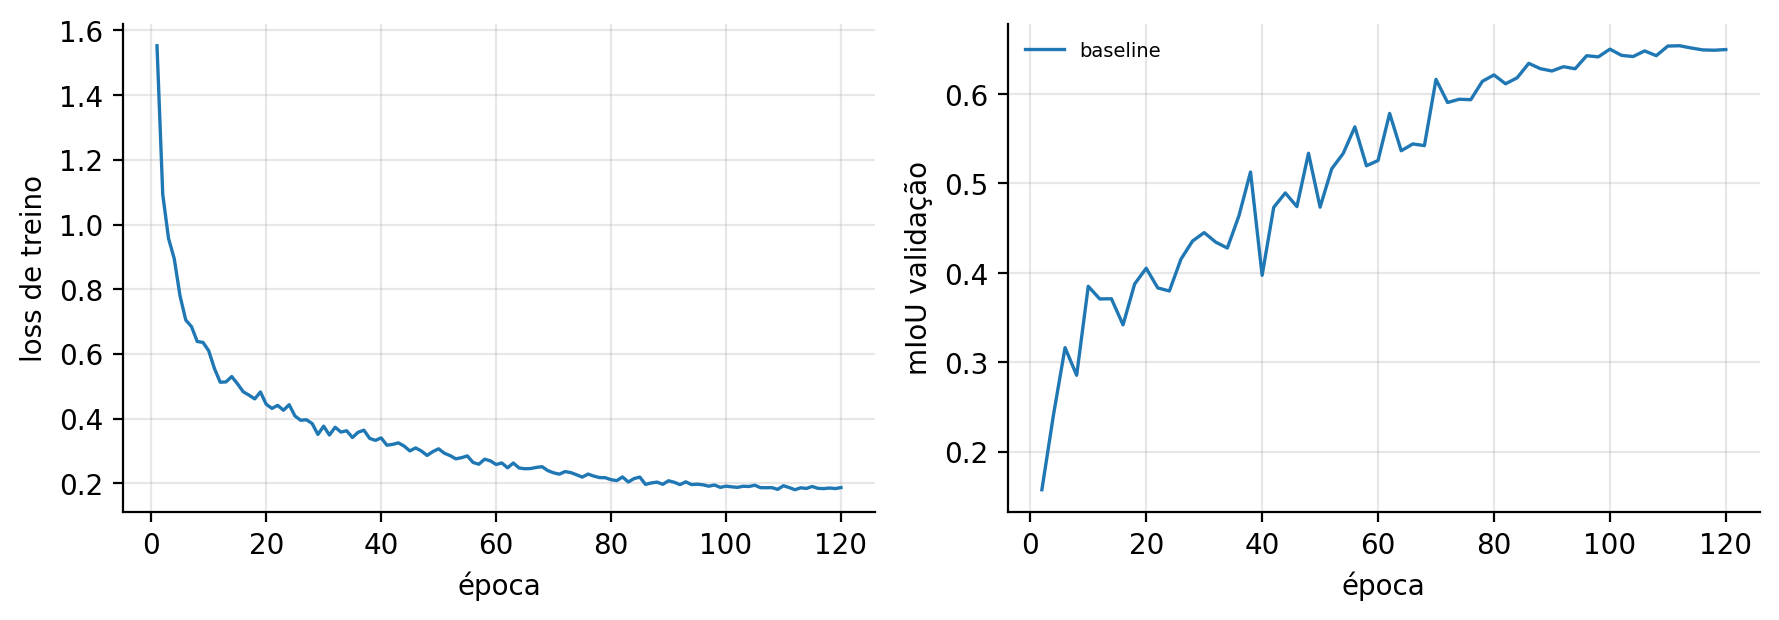
\includegraphics[width=\columnwidth]{fig_curvas_baseline.png}
\fbox{\parbox[c][2.6cm][c]{0.94\columnwidth}{\centering\small
\preencher{fig\_curvas\_baseline.png: loss de treino e mIoU de validação por época}}}
\caption{Curvas de treino do baseline.}
\label{fig:prelim}
\end{figure}

\begin{figure}[h]
\centering
% 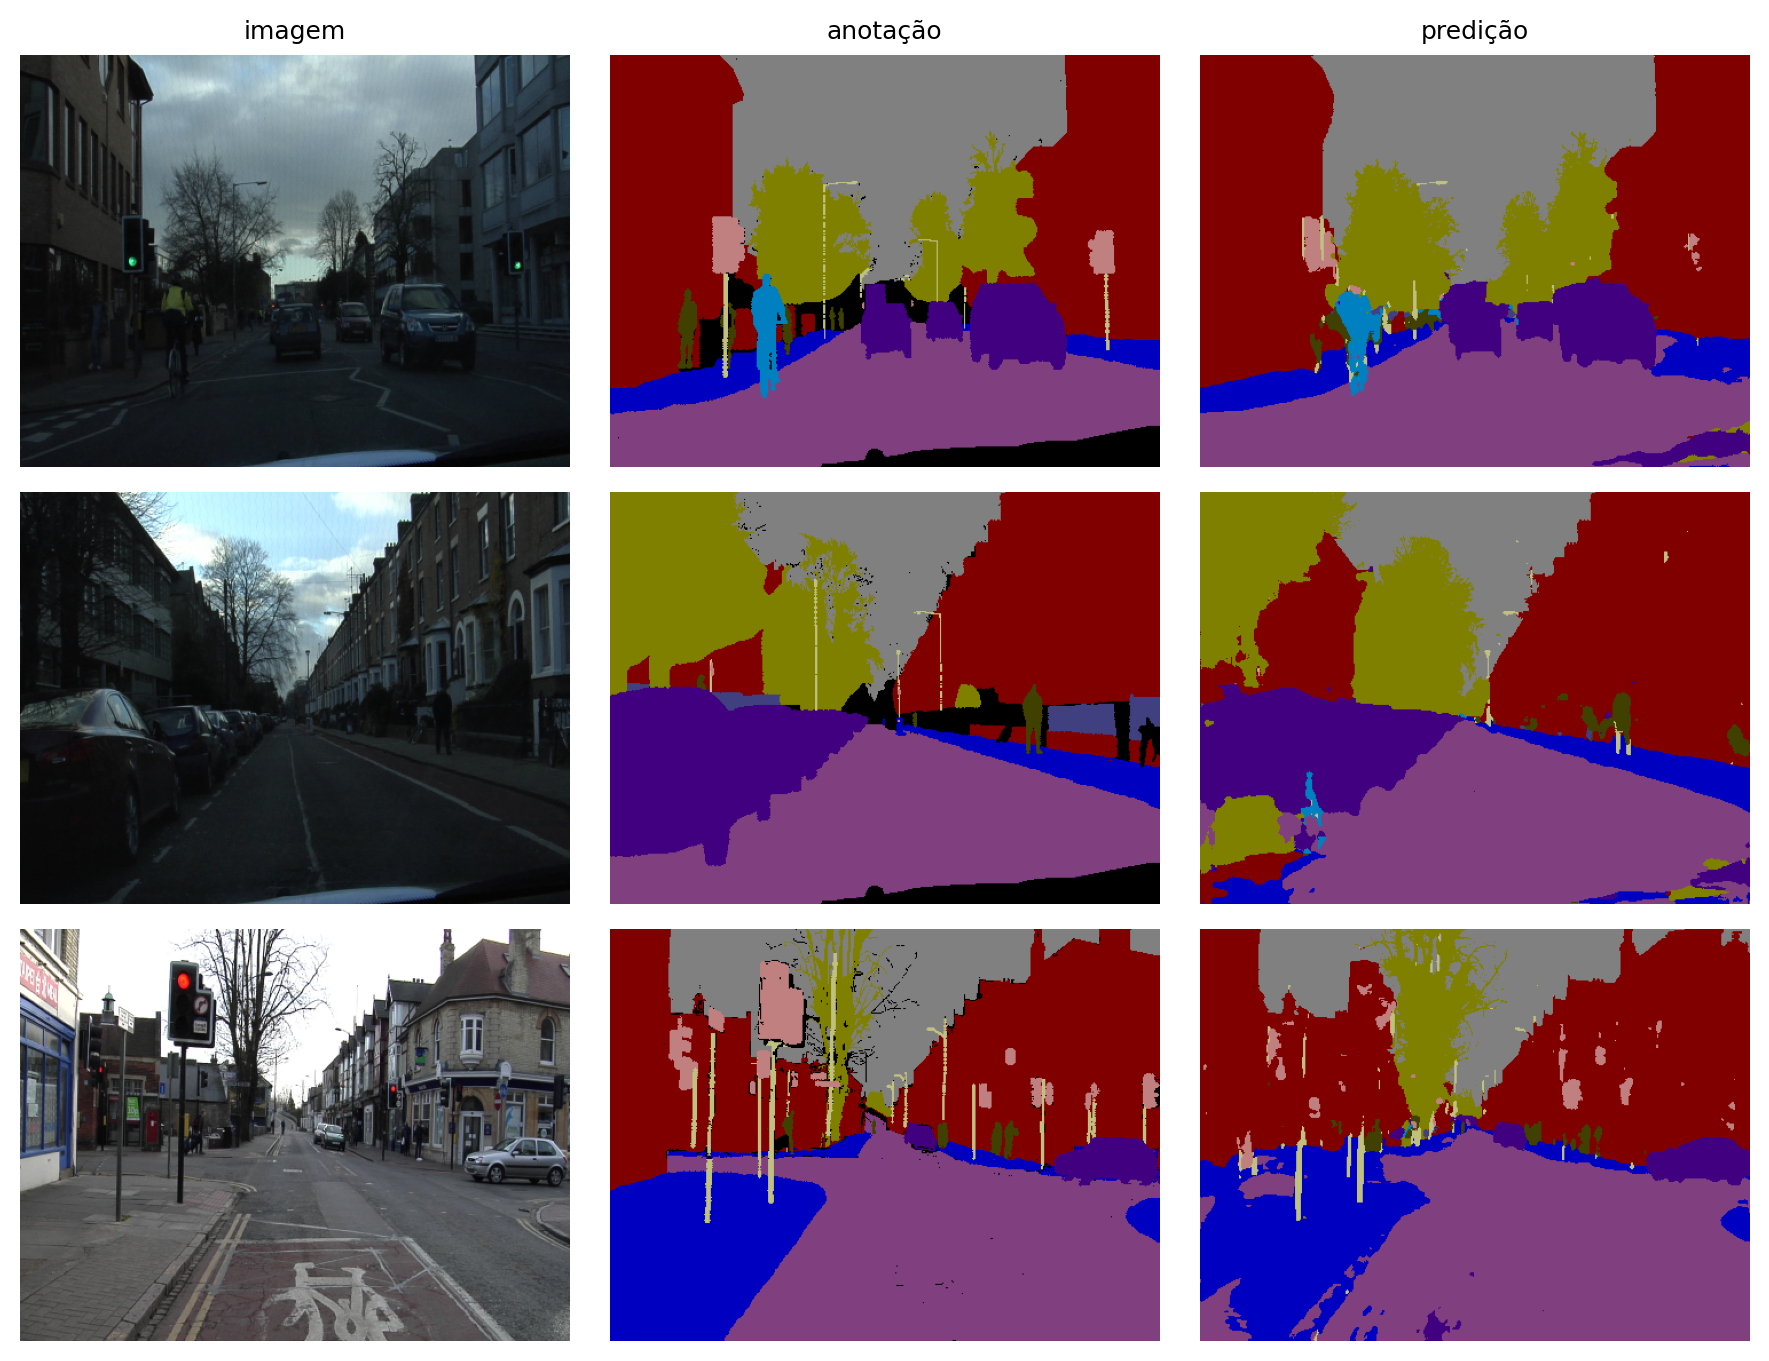
\includegraphics[width=\columnwidth]{fig_exemplos_baseline.png}
\fbox{\parbox[c][3.6cm][c]{0.94\columnwidth}{\centering\small
\preencher{fig\_exemplos\_baseline.png: imagem | anotação | predição (3 exemplos do teste)}}}
\caption{Exemplos qualitativos do baseline no conjunto de teste.}
\label{fig:exemplos}
\end{figure}

\textbf{Leitura inicial:} \preencher{2--3 frases: o modelo convergiu? há sinal de
overfitting? quais classes falham e por quê (tamanho, frequência)?} Como referência,
a U-Net do zero nessa divisão tende a ficar abaixo de modelos pré-treinados; esperamos
mIoU na faixa de 0,50--0,60.

\section{Próximos passos e riscos}
\begin{itemize}
  \item Rodar as variantes de Q1--Q3 com 3 seeds e consolidar as tabelas.
  \item \textbf{Risco:} diferenças entre variantes menores que a variação entre
  seeds; nesse caso, reportamos a ausência de efeito em vez de forçar conclusões.
  \item \textbf{Risco:} cota de GPU; mitigado por checkpoints retomáveis e Q4 opcional.
\end{itemize}

\begingroup\small
\renewcommand{\section}[2]{\vspace{2pt}\noindent\textbf{Referências}\par}
\begin{thebibliography}{9}\setlength{\itemsep}{0pt}
\bibitem{ronneberger} O.~Ronneberger, P.~Fischer, T.~Brox. U-Net: Convolutional networks for
biomedical image segmentation. \emph{MICCAI}, 2015.
\bibitem{camvid} G.~Brostow, J.~Fauqueur, R.~Cipolla. Semantic object classes in video:
a high-definition ground truth database. \emph{Pattern Recognition Letters}, 2009.
\bibitem{segnet} V.~Badrinarayanan, A.~Kendall, R.~Cipolla. SegNet: A deep convolutional
encoder-decoder architecture for image segmentation. \emph{IEEE TPAMI}, 2017.
\bibitem{milletari} F.~Milletari, N.~Navab, S.-A.~Ahmadi. V-Net: Fully convolutional neural
networks for volumetric medical image segmentation. \emph{3DV}, 2016.
\bibitem{eigen} D.~Eigen, R.~Fergus. Predicting depth, surface normals and semantic labels
with a common multi-scale convolutional architecture. \emph{ICCV}, 2015.
\end{thebibliography}
\endgroup

\end{document}
